\documentclass[a4paper,10pt]{article}

%%%% PRATIQUE POUR LES ALINEAS CHIANTS
\usepackage{indentfirst}

%%%% POUR L'OPTION LABEL= %%%
\usepackage{enumitem}

\setlength{\parindent}{30pt}
\setlength{\parskip}{1ex}
\setlength{\textwidth}{15cm}
\setlength{\textheight}{24cm}
\setlength{\oddsidemargin}{0.2cm}
\setlength{\evensidemargin}{-.7cm}
\setlength{\topmargin}{-.5in}

\usepackage{graphicx}
\usepackage{titling}
\usepackage{listings}
\lstset{%
  basicstyle=\scriptsize\sffamily,%
  commentstyle=\footnotesize\ttfamily,%
  frameround=trBL,
  frame=single,
  breaklines=true,
  showstringspaces=false,
  numbers=left,
  numberstyle=\tiny,
  numbersep=10pt,
  keywordstyle=\bf
}
\newcommand{\subtitle}[1]{%
  \posttitle{%
    \par\end{center}
    \begin{center}\large#1\end{center}
    \vskip0.5em}%
}
\title{\textbf{Low level inputs/outputs}}
\subtitle{M1 MoSIG : Operating Systems}
\author{Poupin Pierre \and Rouby Thomas}
\date{18/11/2014}

\begin{document}
\maketitle

\section{Introduction}

Architecture of a typical device :

\begin{figure}[h!]
  \begin{center}
    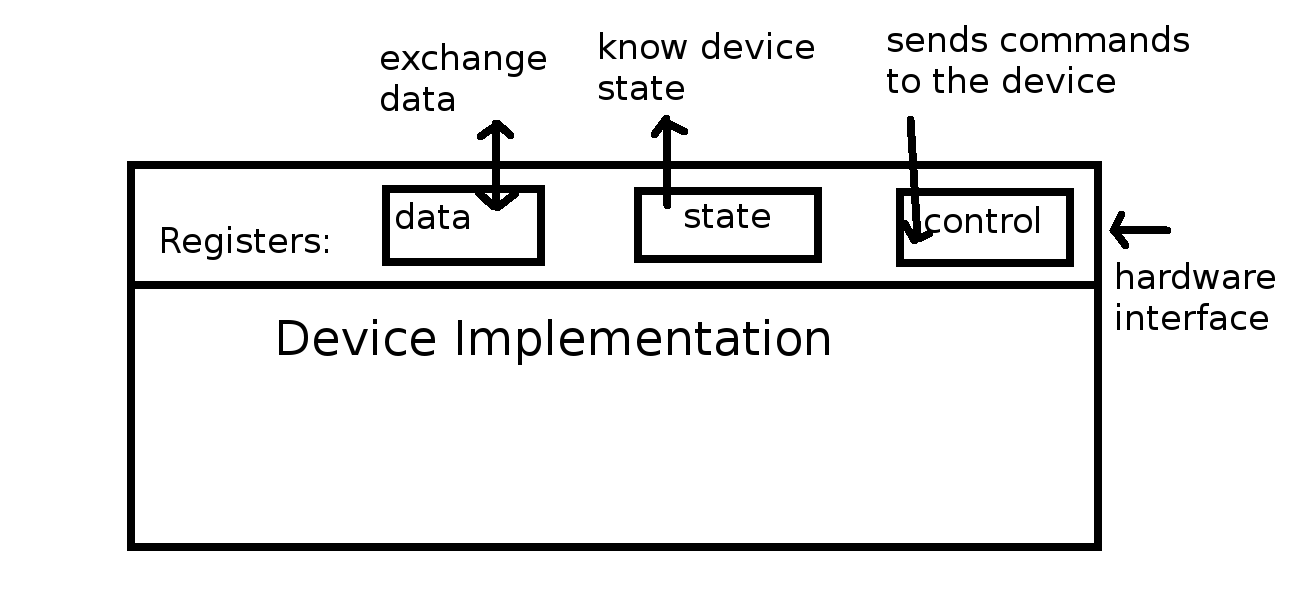
\includegraphics[width=0.8\textwidth]{architecture_device.png}
    \label{Architecture of a typical device}
  \end{center}
\end{figure}
This general scheme applies to : hard drives, printers, mouses...


Computer layout :
\begin{figure}[h!]
  \begin{center}
    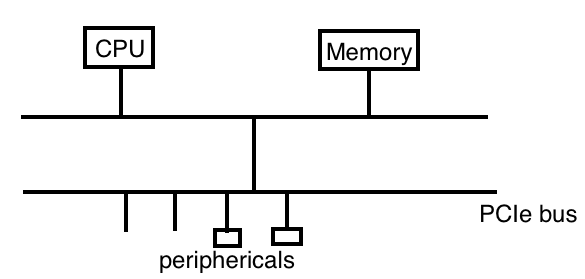
\includegraphics[width=0.8\textwidth]{computer_layout.png}
    \label{fig:1}
  \end{center}
\end{figure}

To access to periphericals, one has to issue either :

\begin{itemize}
  \item special instructions to write to one of the I/O registers of periphericals.
  A port is provided which is the target device.
  
  \item memory access ... . The address space is divided into :
  \begin{itemize}
    \item  main memory
    \item 16 registers of periphericals
  \end{itemize}
\end{itemize}

Basic exchange with a peripherical :

\begin{verbatim}
  while(read(status) == busy) 
  {}
  write(data,some_data);
  write(control,some_command);
  while(read(status)==busy) 
  {}
\end{verbatim}



\section{Device Driver}

The OS would rather handle generic periphericals: for instance, a storage device should look like a sequence of data block

\begin{table}[h]
\begin{tabular}{llllllll}
0                      & 1                     & 2                     & 3                     & 4                     & 5                     & 6                     & 7                     \\ \hline
\multicolumn{1}{|l|}{} & \multicolumn{1}{l|}{} & \multicolumn{1}{l|}{} & \multicolumn{1}{l|}{} & \multicolumn{1}{l|}{} & \multicolumn{1}{l|}{} & \multicolumn{1}{l|}{} & \multicolumn{1}{l|}{} \\ \hline
\end{tabular}
\end{table}
%place table here

Along with two properties :
\begin{itemize}
  \item read(int num\_block, void *result);
  \item write(int num\_block, void *result);
\end{itemize}

A driver is a piece of the OS that provides that kind of abstraction for a specific device type.

\textbf{Example:}

An IDE driver, writing to the disk looks like :
\begin{itemize}
  \item loop waiting for disk availability.
  \item write the block number (28 bits) and the drive number into 4 controls registers.
  \item wait for device availability for data transfer
  \item transfer the data :
  \begin{itemize}
    \item write a data piece (usually 4 bytes) to the data register
    \item write a signal to the command register
    \item wait for completion (polling the status register)
  \end{itemize}
  Repeat until all the data is transfered.
  \item wait for the completion of the operation
  \item report a possible error
\end{itemize}

\begin{figure}[h!]
  \begin{center}
    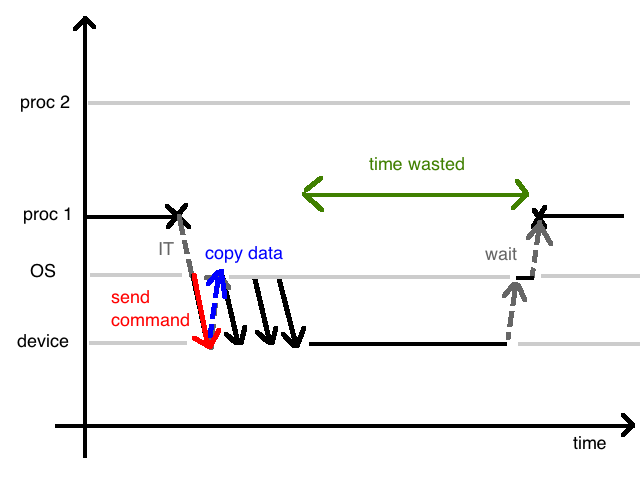
\includegraphics[width=0.8\textwidth]{resources_wasted.png}
    \label{fig:2}
  \end{center}
\end{figure}

\section{Improving resources utilization}
Devices are usually much slower than CPU, We can improve resources utilization, by avoiding active wait.

\subsection{Poll on a regular basis}

\begin{figure}[h!]
  \begin{center}
    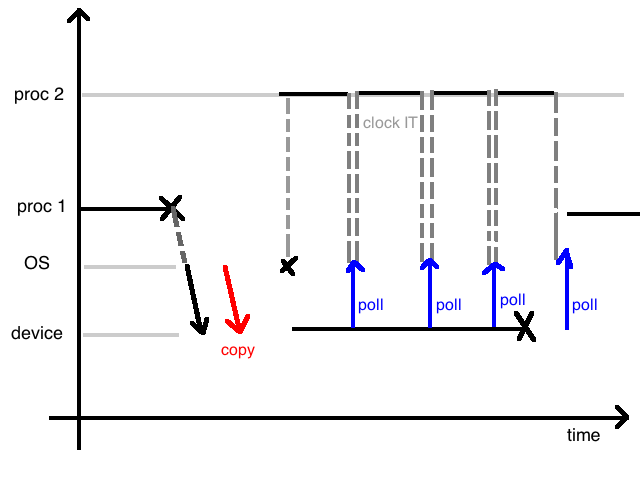
\includegraphics[width=0.8\textwidth]{poll.png}
    \label{fig:3}
  \end{center}
\end{figure}

Issues :

\begin{itemize}
  \item Several polls to the device
  \item The device is not used between the completion of the request and the next poll.
\end{itemize}

\subsection{Use Interrupts}

Now the device has the capacity to raise an interrupt (typically at request completion).

\begin{figure}[h!]
  \begin{center}
    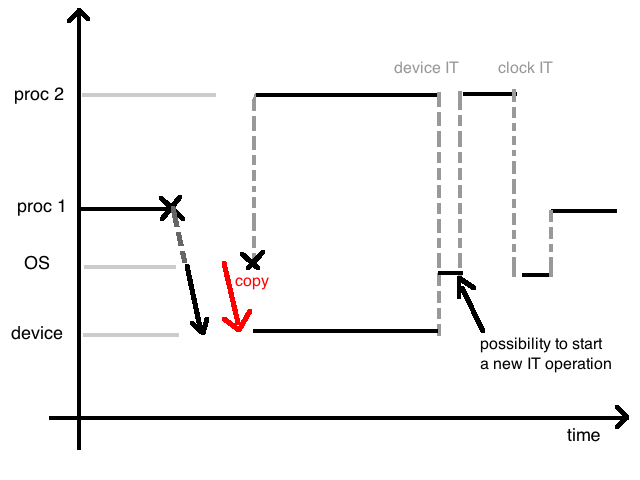
\includegraphics[width=0.8\textwidth]{interrupt.png}
    \label{fig:4}
  \end{center}
\end{figure}

Issues : The CPU is not used efficiently during the copy.

\subsection{Use DMA}

\begin{figure}[h!]
  \begin{center}
    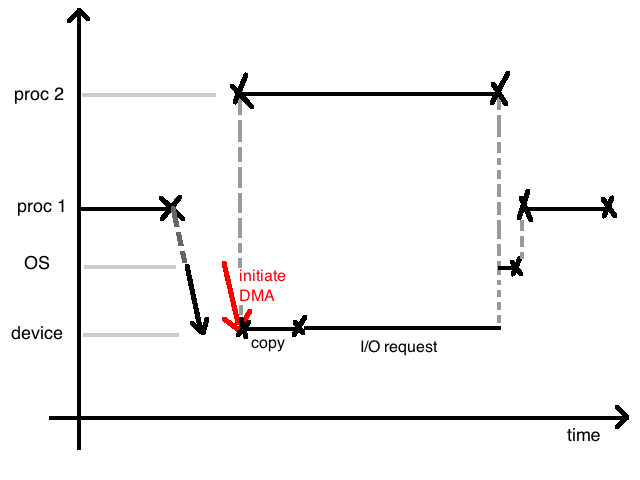
\includegraphics[width=0.65\textwidth]{dma.png}
    \caption{DMA}
    \label{fig:5}
  \end{center}
\end{figure}

DMA stands for Direct Memory Access, it has to be handled both by :
\begin{itemize}
  \item the memory controller
  \item the device
\end{itemize}

It let a device exchange data blocks with the memory without the need of the CPU.
The CPU just has to initiate the access.


DMA is used for fast devices :
\begin{itemize}
  \item hard disks
  \item CD Roms
  \item graphic accelerator
\end{itemize}

\section{Up to the user interface}

\begin{figure}[h!]
  \begin{center}
    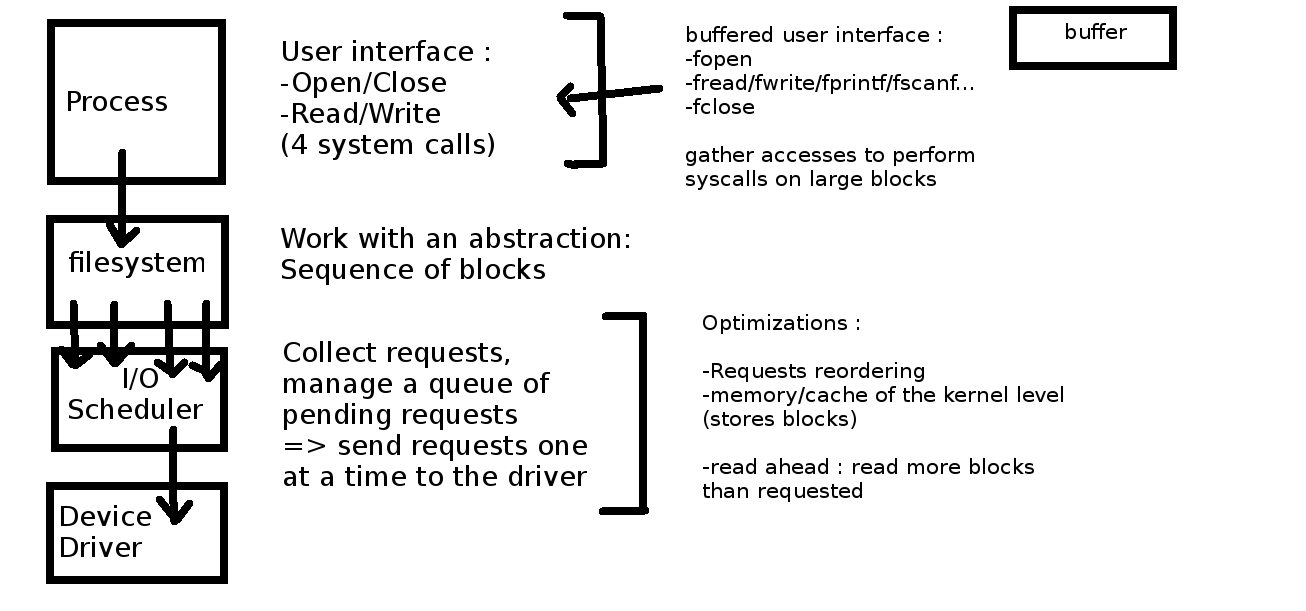
\includegraphics[width=\textwidth]{user_interface.png}
    \label{fig:6}
  \end{center}
\end{figure}

\end{document}
